%%
%% Author: dariochinelli
%% 2020-09-29
%%


\section{Principio di indeterminazione di Heisemberg}

Il principio di Heisemberg è costituito da due parti:
la prima parte riguarda la misura simultanea di momento e posizione di una particella.
Un esperimento non può determinare il valore esatto di una componente del momento $p_x$ e anche il valore esatto della $x$, la precisione della misura è limitata dal processo stesso della misura per cui
\begin{equation}
\begin{split}
& \Delta p_x \Delta x \ge \frac{ \hbar}{2 } \\
& \hbar = \frac{ h}{2\pi }
\end{split}
\end{equation}
È implicato il prodotto tra le incertezze per cui se l'incertezza sul momento è nulla, l'incertezza sulla posizione sarà infinita: $\Delta p_x = 0 \Rightarrow \Delta x = \infty$
Valgono le espressioni analoghe per le altre componenti
\begin{equation}
\begin{split}
& \Delta p_y \Delta y \ge \frac{ \hbar}{2 } \\
& \Delta p_z \Delta z \ge \frac{ \hbar}{2 }
\end{split}
\end{equation}
La seconda parte riguarda una relazione analoga tra l'energia ed il tempo richiesto per effettuare la misura:
\begin{equation}
\Delta E \Delta t \ge \frac{\hbar}{2}
\end{equation}
Il fatto che la costante di Planck sia tanto piccolo non permette di vedere questi fenomeni nella vita ordinaria, quindi la fisica classica è ancora valida per descrivere oggetti macroscopici.


\paragraph{Esperimento concettuale di Bohr}
Cosa accade quando si desidera misurare con grandissima precisione la posizione di un elettrone?
Si può utilizzare un "microscopio" e illuminare l'elettrone con un fotone per poi vederlo mediante scattering Compton.
Osservare la particella non è un'azione priva di conseguenze poiché illuminandolo si produce un'interazione fotone-elettrone.
Tale perturbazione può essere ridotta al minimo, ma non eliminata, mandando un solo fotone per volta.
Si noti comunque che anche in meccanica classica, in un certo senso, l'osservatore disturba il moto del corpo in esame: se si studia il moto di un pianeta la massa dell'osservatore da luogo ad un'interazione gravitazionale,
ma data la piccolezza della massa di questi rispetto al pianeta, e tale interferenza è trascurabile.
In figura \ref{esp_bohr} è rappresentato l'esperimento mentale proposto da Bohr.
\begin{figure}[h]
\centering
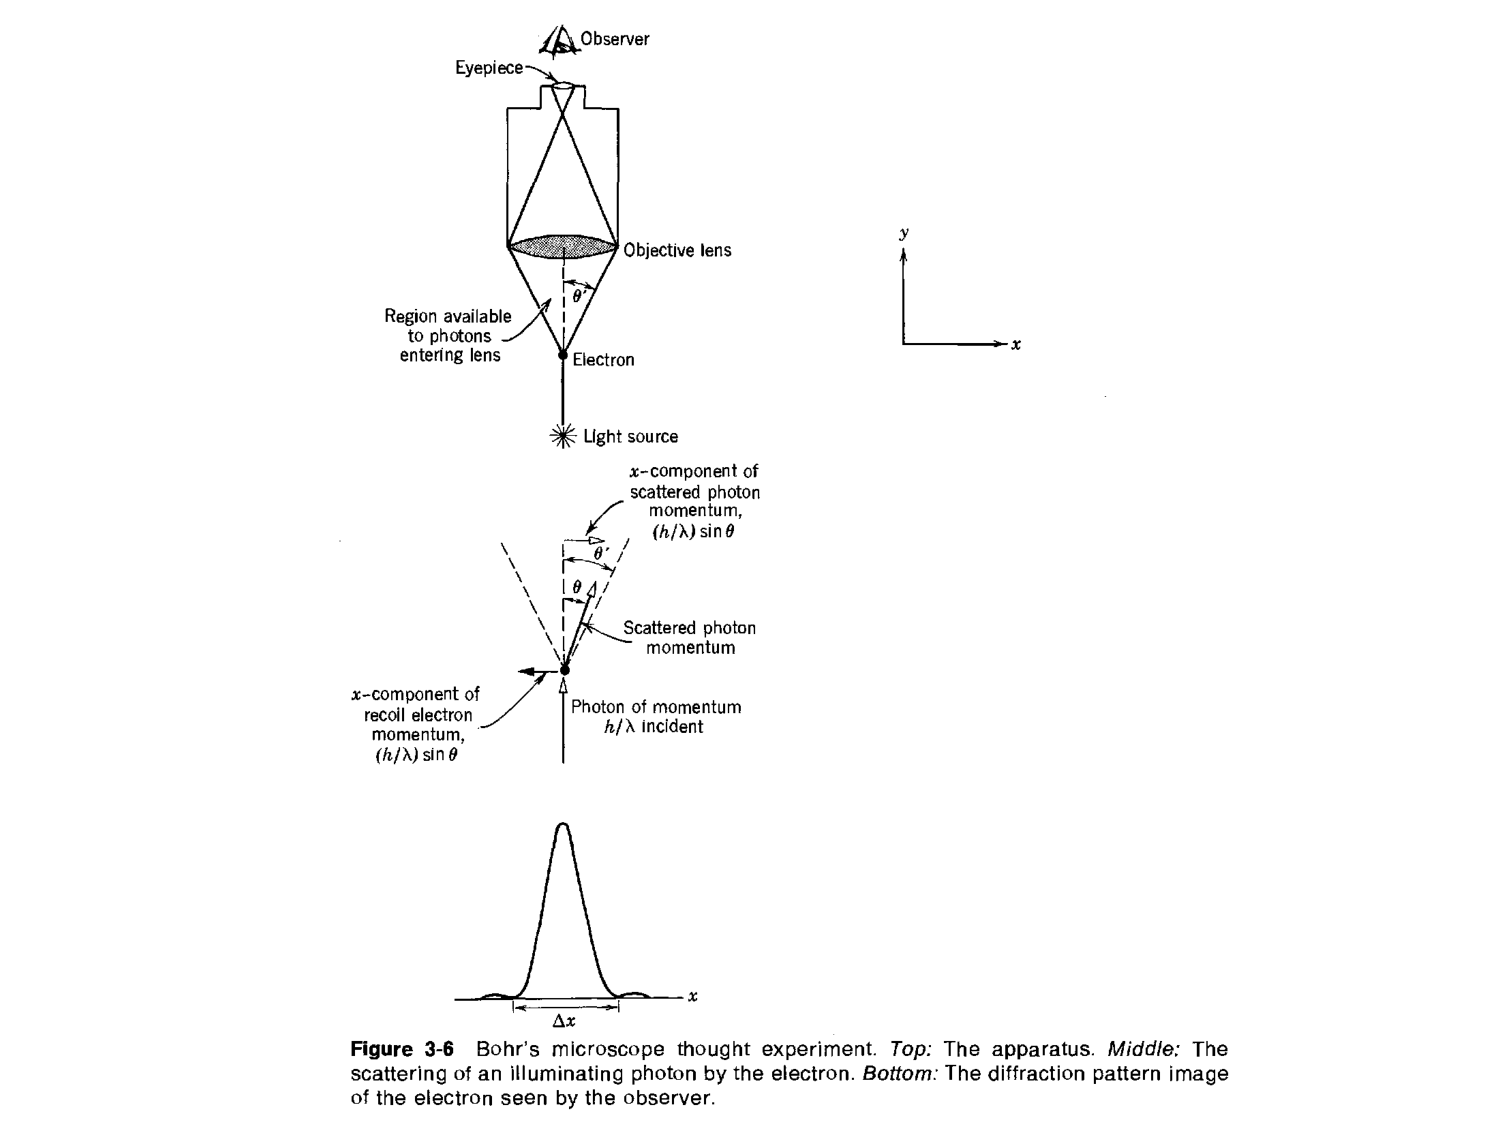
\includegraphics[scale=0.5]{/microsopio_bohr}
\caption{Schema dell'esperimento di Bohr}
\label{esp_bohr}
\end{figure}

\paragraph{momento angolare} Il momento angolare del fotone è dato dalla solita equazione
\begin{equation}
\begin{split}
p & = \frac{h}{\lambda} \\
p_x & = \frac{h}{\lambda} \sin\theta'
\end{split}
\end{equation}
e tale momento angolare potrà variare da $+P\sin \theta '$ a $-P \sin \theta '$ allora
\begin{equation}
\Delta p_x = 2p \sin \theta ' = 2(\frac{h }{\lambda }) \sin \theta '
\end{equation}
è l'incertezza sulla componente $x$ del momento angolare del fotone $p_x$, che, per la conservazione del momento angolare, sarà uguale a quella dell'elettrone.

\paragraph{posizione} Cosa si può dire sulla posizione $x$ dell'elettrone?
L'immagine di un microscopio è un reticolo di diffrazione, allora possiamo considerare l'ampiezza del massimo centrale di diffrazione come misura dell'incertezza della posizione del fotone, e anche questa misura è analoga per l'elettrone
\begin{equation}
\begin{split}
\Delta x = \frac{\lambda}{\sin \theta '}
\end{split}
\end{equation}

Per ridurre l'incertezza sul momento dovrei aumentare la $\lambda$, viceversa per ridurre l'incertezza sulla posizione dovrei aumentare la $\lambda$, ovvero l'esatto contrario.
Facendo il prodotto tra le due incertezze trovo:
\begin{equation}
\Delta p_x \Delta x = (\frac{2h}{\lambda} \sin \theta ')(\frac{\lambda}{\sin \theta '}) = 2h > \frac{\hbar}{2}
\end{equation}
che non è propriamente il valore previsto dal Principio di Indeterminazione ma è comunque una costante.
Significa che far interferire un fotone con l'elettrone perturba la misura in un modo che non posso evitare, ovvero il PdI riguarda strettamente l'incapacità di una misurazione infinitamente precisa.

Per quanto riguarda la seconda parte, scriviamo l'energia del fotone ed il tempo necessario per la misura
\begin{equation}
\begin{split}
& E = \frac{ p_x^2}{2m } \\
\Rightarrow & \Delta E = \Bigl(  \frac{ p_x}{m }  \Bigr) \Delta p_x = v_x \Delta p_x \\
& \Delta x = v_x \Delta t \\
\Rightarrow & \Delta t = \frac{ \Delta x}{v_x }
\end{split}
\end{equation}
dove $v_x$ è la velocità, allora si trova
\begin{equation}
\begin{split}
& \Delta E \Delta t = \Delta p_x \Delta x \\
& \Delta E \Delta t = 2h \ge \frac{ \hbar}{2 }
\end{split}
\end{equation}
in modo analogo all'equazione precedente, ovvero l'osservatore modifica in modo non trascurabile ed inevitabile l'osservato.


\paragraph{Esempio} La velocità di un proiettile di massa $m_p = \SI{50}{g}$ e di un elettrone di massa
$m_e = \SI{9.1e-28}{g}$ sono misurate contemporaneamente e sono uguali $V = \SI{300}{m/s}$, con un'incertezza di $10^{-4}$.
Con quale precisione posso localizzare la posizione di entrambi, se la posizione è misurata simultaneamente con la velocità nello stesso esperimento?

Considero solo la direzione lungo l'asse $x$.
 
\underline{Per il proiettile:}
\begin{equation}
\begin{split}
& p = m v = \SI{5e-2}{kg} \cdot \SI{300}{m/s} = \SI{15}{kg.m/s} \\
& \Delta p = \SI{e-4}{} \cdot \SI{15}{kg.m/s} = \SI{1.5e-3}{kg.m/s} \\
& \Delta x = \frac{ h}{4\pi \Delta p } = \frac{ \SI{6.6e-34}{j.s}}{4\pi \cdot \SI{1.5e-3}{kg.m/s} } = \SI{3e-32}{m}
\end{split}
\end{equation}
che sono rispettivamente l'incertezza sulla quantità di moto e l'incertezza sulla posizione del proiettile, notiamo che l'incertezza rispetto alle dimensioni del proiettile ($\SI{e-2}{m}$) è pressoché trascurabile.

\underline{Per l'elettrone:}
\begin{equation}
\begin{split}
& p = m v = \SI{9.1e-31}{kg} \cdot \SI{300}{m/s} = \SI{2.7e-28}{kg.m/s} \\
& \Delta p = \SI{e-4}{} \cdot \SI{2.7e-28}{kg.m/s} = \SI{2.7e-32}{kg.m/s} \\
& \Delta x = \frac{ h}{4\pi \Delta p } = \frac{ \SI{6.6e-34}{j.s}}{4\pi \cdot \SI{2.7e-32}{kg.m/s} } = \SI{2e-3}{m} = \SI{0.2}{cm}
\end{split}
\end{equation}
che sono rispettivamente l'incertezza sulla quantità di moto e l'incertezza sulla posizione dell'elettrone, rispetto alle \textit{dimensioni} di un elettrone i 2 mm di incertezza rendono impossibile localizzarlo con precisione.

\paragraph{Derivazione del principio di indeterminazione}
Ricaviamo ora le relazioni del principio di indeterminazione combinando le equazioni di De Broglie e di Einstein, utilizzando le proprietà universali delle onde e le trasformate di Fourier, quindi
\begin{equation}
E = h \nu \quad\quad\quad p = \frac{ h}{\lambda }
\label{dualita_oc}
\end{equation}
Per ottenere una funzione d'onda che sia diversa da zero solo dove è localizzata la particella devo considerare un gruppo di onde e non una sola onda monocromatica.
Ad esempio un gruppo di due onde è così costruito
\begin{equation}
\begin{split}
& \Psi(x,t) = \Psi_1(x,t) + \Psi_2(x,t) \\
& \Psi_1(x,t) = \sin \Bigl[  2\pi (kx -\nu t)  \Bigr] \\
& \Psi_1(x,t) = \sin \Bigl[  2\pi ((k + dk) x - (\nu +d\nu) t)  \Bigr]
\end{split}
\label{eq_onde_gen}
\end{equation}

\begin{figure}[h]
\centering
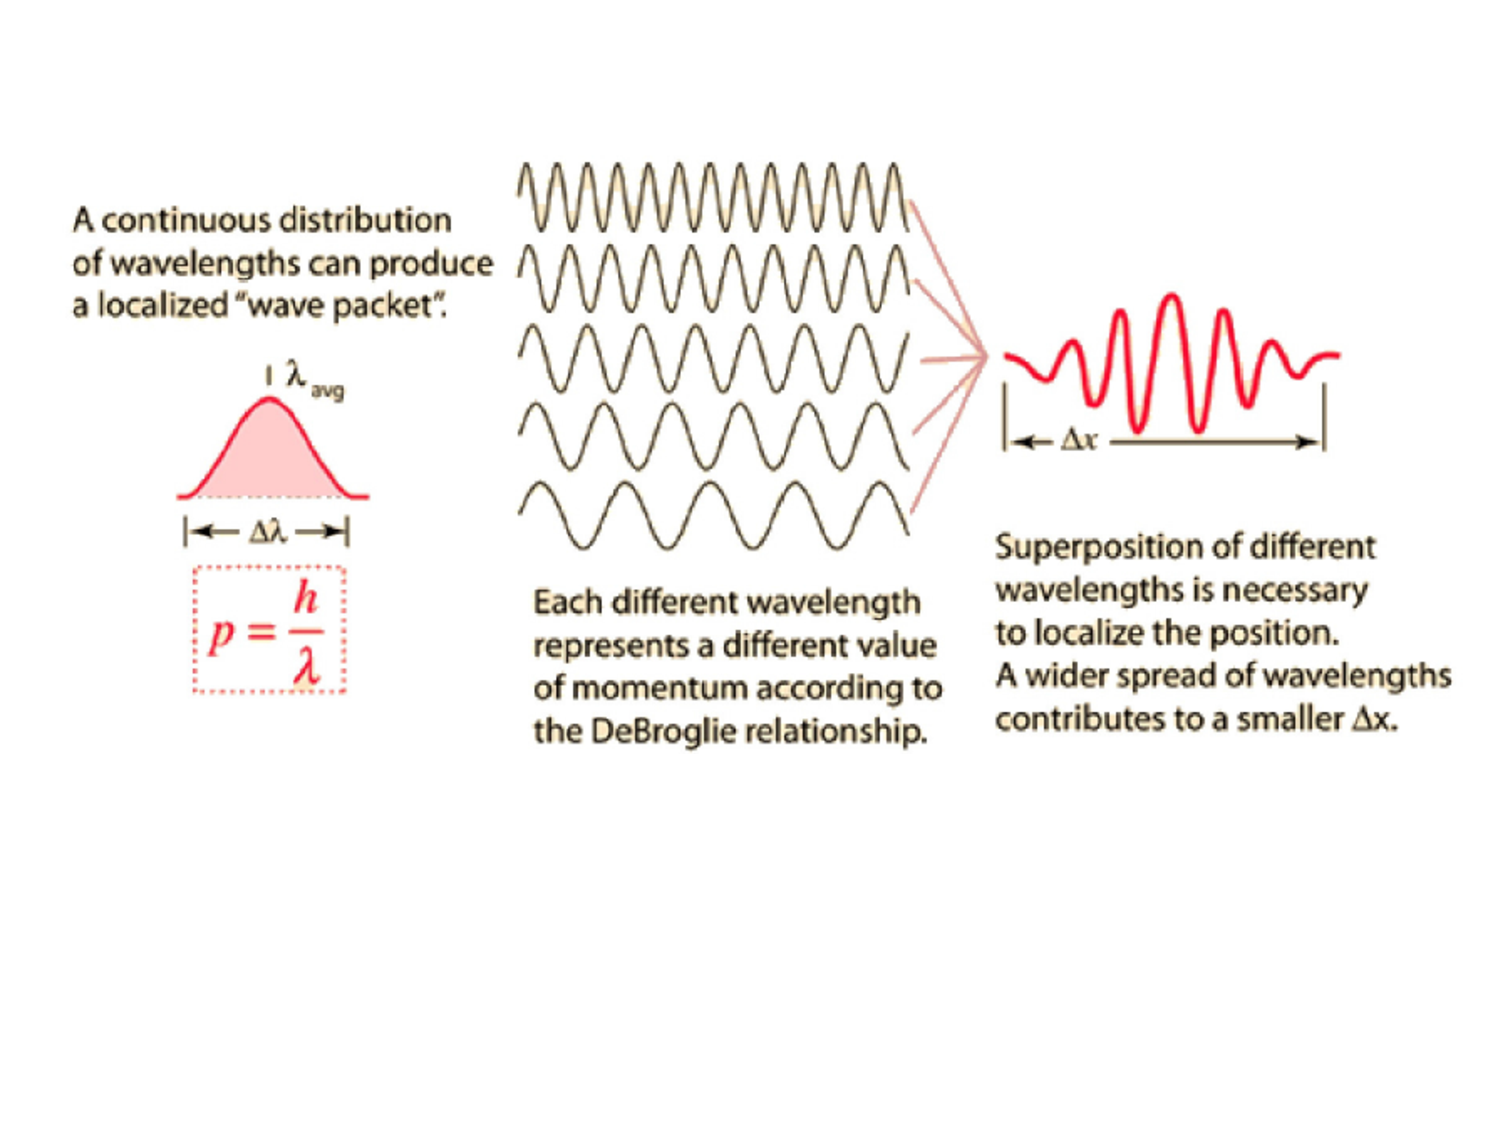
\includegraphics[scale=0.5]{/wave_packet}
\caption{Come produrre un'onda localizzata}
\end{figure}

Per localizzare maggiormente lo spazio in cui trovare la particella $\Delta x$devo aumentare il range di $\Delta k$.

\paragraph{Analisi di Fourier} 
queste sono le relazioni universali per tutte le onde
\begin{equation}
\begin{split}
& \Delta x \Delta k \ge \frac{ 1}{4\pi } \\
& \Delta t \Delta \nu \ge \frac{ 1}{4\pi }
\end{split}
\label{eq_univ}
\end{equation}
Ciò deriva dallo studio della velocità di gruppo delle onde.

La velocità di propagazione di un'onda è $W=\lambda \nu$ per De Broglie è $$W = \lambda \nu = \frac{h}{p} \frac{E}{h} = \frac{E}{p}$$
Assumendo che la particella si muova a velocità non relativistiche $V$ in una regione definita, si ottiene che:
\begin{equation}
W = \frac{E}{p} = \frac{1}{2} \frac{m V^2}{m V} = \frac{V}{2}
\end{equation}
tuttavia questo risultato non è buono poiché sembra affermare che le onde di materia non siano capaci di "tenere il passo" rispetto alla particella...

Si immagini che la particella si muova libera lungo l'asse x, e si associ a tale moto un'onda di materia. Al tempo $t=0$ si registra la sua ampiezza.
Si associa quindi una funzione $\Psi (x,t)$.
Consideriamo ora la velocità di gruppo di tali onde, data dalla $g=\frac{d \nu}{d k}$ con $k= \lambda^{-1}$ e si consideri quindi la generica onda.

Si può trattare un gruppo di onde come una semplice somma di più onde, come in equazione \ref{eq_onde_gen}, da cui si ottiene 
\begin{equation}
\Psi (x, t) = 2 \cos [ 2 \pi ( \frac{dk}{2} x - \frac{d\nu}{2} t ) ] \sin [ 2\pi ( \frac{2k + dk}{2} x - \frac{2\nu + d\nu}{2} t ) ]  
\end{equation}
e se $ d\nu \ll 2\nu $ e $ dk \ll 2k $
\begin{equation}
 \Psi (x, t) = 2 \cos [ 2 \pi ( \frac{dk}{2} x - \frac{d\nu}{2} t ) ] \sin [ 2 \pi ( k x - \nu t )] 
\end{equation}

Dunque due onde con una lieve differenza di frequenza e di lunghezza d'onda interferiscono e producono una successione di gruppi che si muovono lungo l'asse $x$.
La velocità $W$ delle onde individuali può essere valutata considerando il secondo fattore di $\Psi (x, t)$, e la velocità $g$ di gruppo può essere trovata dal primo fattore.
Ciò non cambia considerando più di due onde.
$$ g = \frac{d\nu}{2}\frac{2}{dk} = \frac{d\nu}{dk} $$
\begin{equation}
\begin{split}
& \nu= \frac{E}{h} \rightarrow d\nu = \frac{d E}{h} \\
& k = \frac{1}{\lambda} = \frac{p}{h} \rightarrow dk=\frac{d p}{h}
\end{split}
\end{equation}
Così si ottiene la velocità di gruppo: 
\begin{equation}
\begin{split}
& g = \frac{d E}{d p} = \frac{m v dv}{m dv} = v \\
& \Rightarrow g = v
\end{split}
\end{equation}
Partendo dalle equazioni \ref{eq_univ} universali delle onde, dalle proprietà delle onde e dalle espressioni \ref{dualita_oc} troviamo il risultato cercato
\begin{equation}
\begin{split}
& \Delta x \Delta k = \Delta x \Delta \frac{1}{\lambda} = \Delta x \Delta \frac{p}{h}  \ge \frac{1}{4\pi} \\
& \Rightarrow \Delta x \Delta p \ge \frac{\hbar}{2} \\
& \Delta t \Delta \nu = \Delta t \Delta \frac{E}{h} \ge \frac{1}{4\pi} \\
& \Rightarrow \Delta t \Delta E \ge \frac{\hbar}{2}
\end{split}
\end{equation}
Ovvero:
\begin{equation}
\begin{split}
& \Delta p \Delta x \ge \frac{\hbar}{2} \\
& \Delta E \Delta t \ge \frac{\hbar}{2}
\end{split}
\end{equation}






